\documentclass[10pt,twocolumn]{article}

% use the oxycomps style file
\usepackage{oxycomps}

% usage: \fixme[comments describing issue]{text to be fixed}
% define \fixme as not doing anything special
\newcommand{\fixme}[2][]{#2}
% overwrite it so it shows up as red
\renewcommand{\fixme}[2][]{\textcolor{red}{#2}}
% overwrite it again so related text shows as footnotes
%\renewcommand{\fixme}[2][]{\textcolor{red}{#2\footnote{#1}}}

% read references.bib for the bibtex data
\bibliography{references}

% include metadata in the generated pdf file
\pdfinfo{
    /Title (Git Tutorial)
    /Author (Runpeng Li)
}

% set the title and author information
\title{Git Tutorial}
\author{Runpeng Li}
\affiliation{Occidental College}
\email{rli3@oxy.edu}

\begin{document}

\maketitle

\section{Prerequisites}

In order to follow along with this tutorial, it is suggested that you have some basic understanding of the command line. Also you will need to have git installed and a GitHub account set up.

\section{What is git}

Git is a robust software development tool for tracking changes in files and sharing them with collaborators. It's distributed, so every developer has a complete history of the code on their own machine.

\section{To Start:}

Let's kick things off by creating a new repository on GitHub. A repository serves as your Git-managed storage, tracking the history and modifications of your files. It's the hub for collaborative work with fellow developers on your project. Here's what it should resemble:

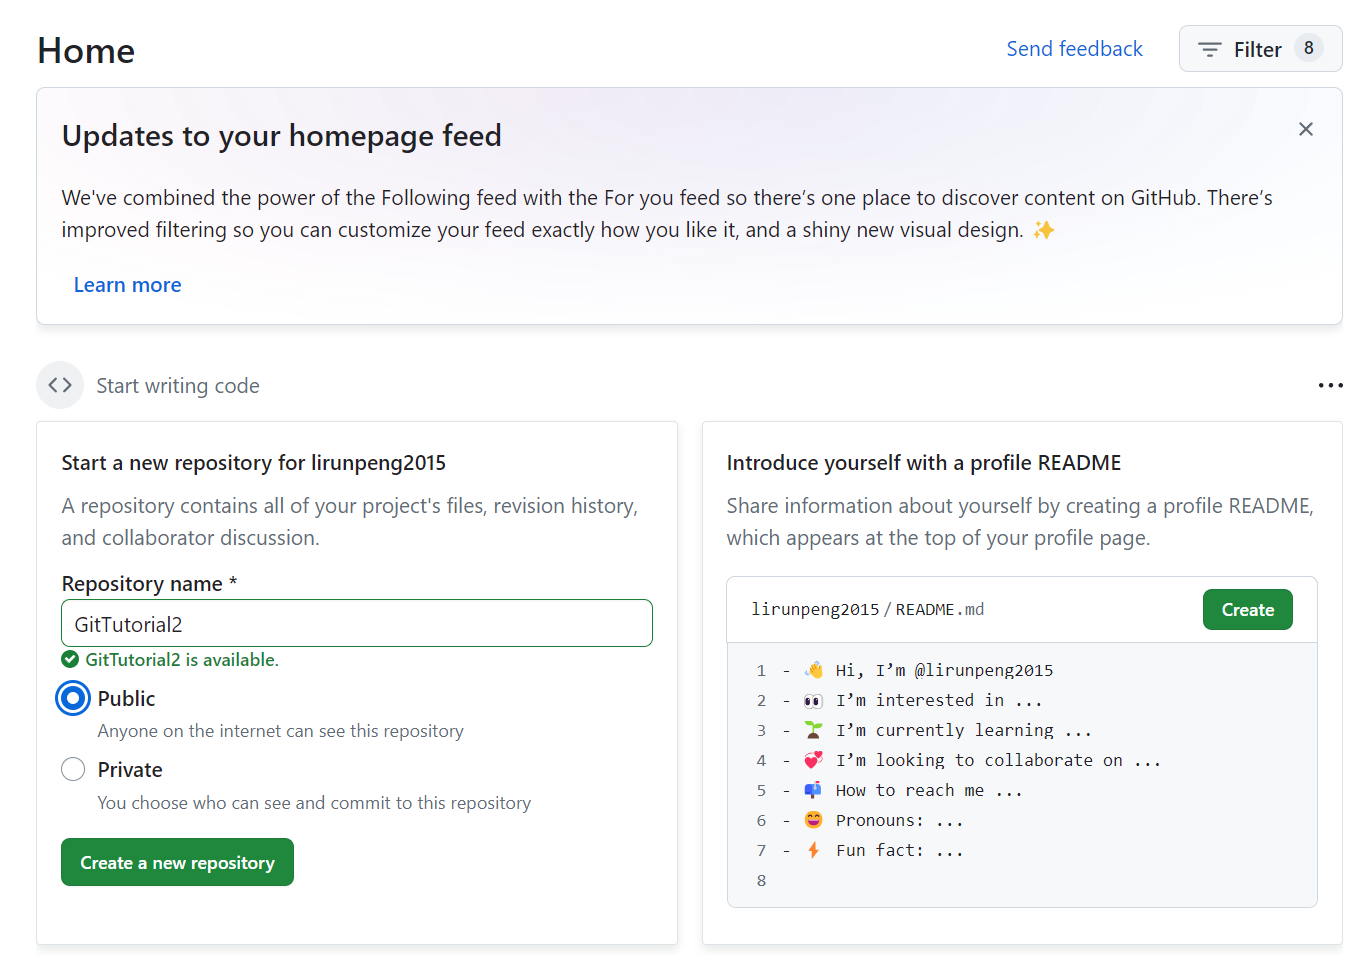
\includegraphics[width = 0.4\textwidth]{Start.png}

After you have created a repository, you can clone it to your computer using this command line: \textbf{git clone[URL]} 

Then you can find and copy the link to the URL of your desire repository on Github by clicking the \textbf{Code} tab. 

\section{Creating File: }

To navigate to and operate within your repository, use the 'cd' command: cd \textbf{*repository name*}. Initially, your repository is empty. Let's begin by creating a Python file using the 'mkdir' command: \textbf{ mkdir *your file name*}. For instance, I named my file hiGit.py.

After successfully creating the file, you can use the 'ls -la' command to view it in the repository. Your output should resemble this:

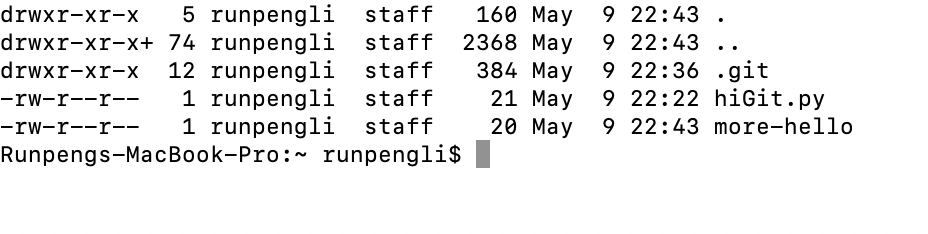
\includegraphics[width = 0.4\textwidth]{Branches.png}


\section{Editing File:}

Now that we've added a Python file to our repository, we can dive into editing it and then commit our initial changes to the repository.

To edit the file, we use the 'vim' command: \textbf{vim *file name*}. This will open a new window. Press the 'i' key first to insert and write code. After making changes, hit the 'escape' key and type \textbf{':wq'} (write and quit) at the bottom to save your edits.

For example, in my hiGit.py file, I added a simple print statement.

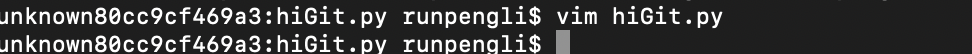
\includegraphics[width = 0.4\textwidth]{Ef.png}
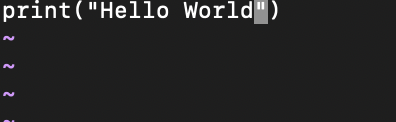
\includegraphics[width = 0.4\textwidth]{EF2.png}



\section{Committing: }

Let's now utilize the \textbf{'git status'} command to display the modifications made to the file.

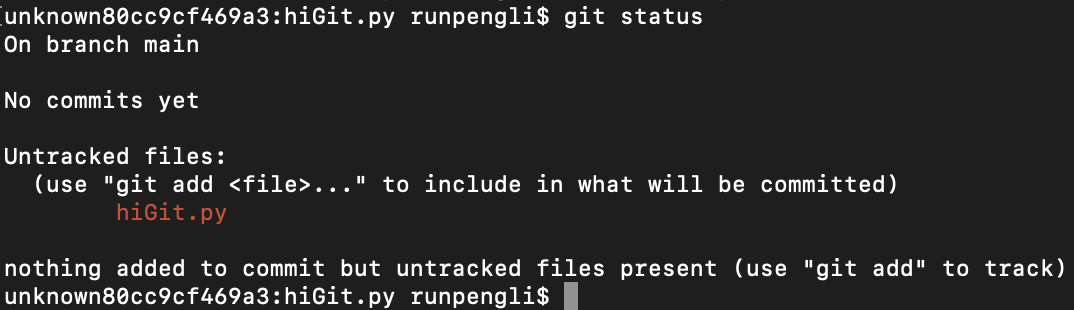
\includegraphics[width = 0.4\textwidth]{Commiting.png}

Upon checking, we observe that an untracked file, hiGit, has been altered.

Our subsequent action involves committing these changes. However, prior to that, we must shift our files to the staging area. The staging area, also referred to as the index, enables us to selectively choose which modifications to include in the subsequent commit. To accomplish this, we use the command: \textbf{'git add -A'} to add all files to the staging area.

Once the file is in the staging area, we can commit it to the repository using: \textbf{'git commit -m "Commit message"}'. The commit message should describe the changes being committed. For instance, I used the message: \textbf{'git commit -m "initial commit"}'.

Upon successful commit, it should appear like this:

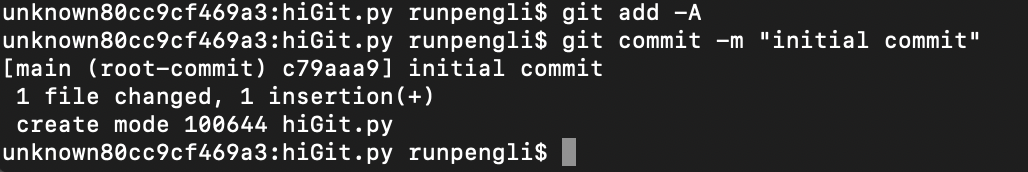
\includegraphics[width = 0.4\textwidth]{Comm2.png}
 
\section{Branches:}

branches in Git. Branches are essential for isolating development tasks such as feature enhancements, bug fixes, or experimenting with new ideas without disrupting the stability of the "main" branch. This feature allows multiple developers to work on different tasks simultaneously within the same project.

To demonstrate the use of branches, let's start by cloning an existing repository into a new one. First, create a new repository named \textbf{byeGit} and clone it locally. Before cloning the old repository into this new one, we should first move into the new repository using the command: \textbf{cd byeGit}. Check for any existing \textbf{.git}directories that could cause a conflict by using the \textbf{ls -a} command. If you find a \textbf{.git} directory, remove it with the command: \textbf{rm -rf} .git to avoid cloning errors.

Next, clone the original repository directly into this new one by using: \textbf{git clone ../GitTutorial2 ..} This action will import all contents, including the \textbf{hiGit.py} file, into \textbf{byeGit}. Proceed to edit \textbf{hiGit.py} within this new repository, perhaps using the vim command to add another print statement.

Now, before pushing any changes to your target repository, you'll need to create a temporary branch in the old repository. Navigate back to the old repository and create a new branch using: \textbf{git checkout -b [temporary branch name]}. Once on the new branch, you can return to the byeGit repository and push the changes.

At this stage, it's also a good idea to create a new permanent branch in the byeGit repository using: \textbf{git branch [new branch name]}, and then switch to it with: \textbf{git checkout [new branch name]}. You can see this new branch listed when you execute: \textbf{git branch}.

\section{Merging}

After making changes on your new branch, consider merging these back to the main branch to integrate your updates. Commit your changes on the new branch, then push them to the original repository using: \textbf{git push -u origin [branch name]}. To merge, switch back to the main branch \textbf{(git checkout main)}, merge the new branch \textbf{(git merge [name of branch])}, and finally, push the merged changes \textbf{(git push origin main)}

\section{Deleting Branches:}.

Once merged, you can delete the obsolete branch with: \textbf{git branch -d [name of branch]}, and also ensure to remove it from the remote repository with: \textbf{git push origin --delete [name of branch]}.

\section{Stashes:}

Lastly, Git stashes are particularly useful for temporarily setting aside modifications that are not ready to be committed. This can be helpful when you need to switch tasks between branches. To demonstrate, make a change to \textbf{hiGit.py}, check its status with \textbf{git status}, and stash the changes with \textbf{git stash}. This will clean your working tree and safely store the changes for later re-application.

This walkthrough provides a practical guide to managing branches, merging, and stashes in Git, tailored specifically to your \textbf{hiGit.py} file and \textbf{byeGit} repository.




\printbibliography

\end{document}  